\chapter{System Design}
\label{ch:design}

\section{System Architecture}

The system is organised as three logical tiers --- an \emph{ingestion
and generation} tier, a \emph{run and verification} tier, and an
\emph{analysis} tier --- that share a persistent store and a job
queue. The tiers correspond respectively to turning a user request
into a plan and runnable code, to executing that code under
supervision and verifying its alignment with the plan, and to
answering the five research questions over the accumulated run
records.

\begin{figure}[htbp]
    \centering
    \begin{subfigure}{\textwidth}
        \centering
        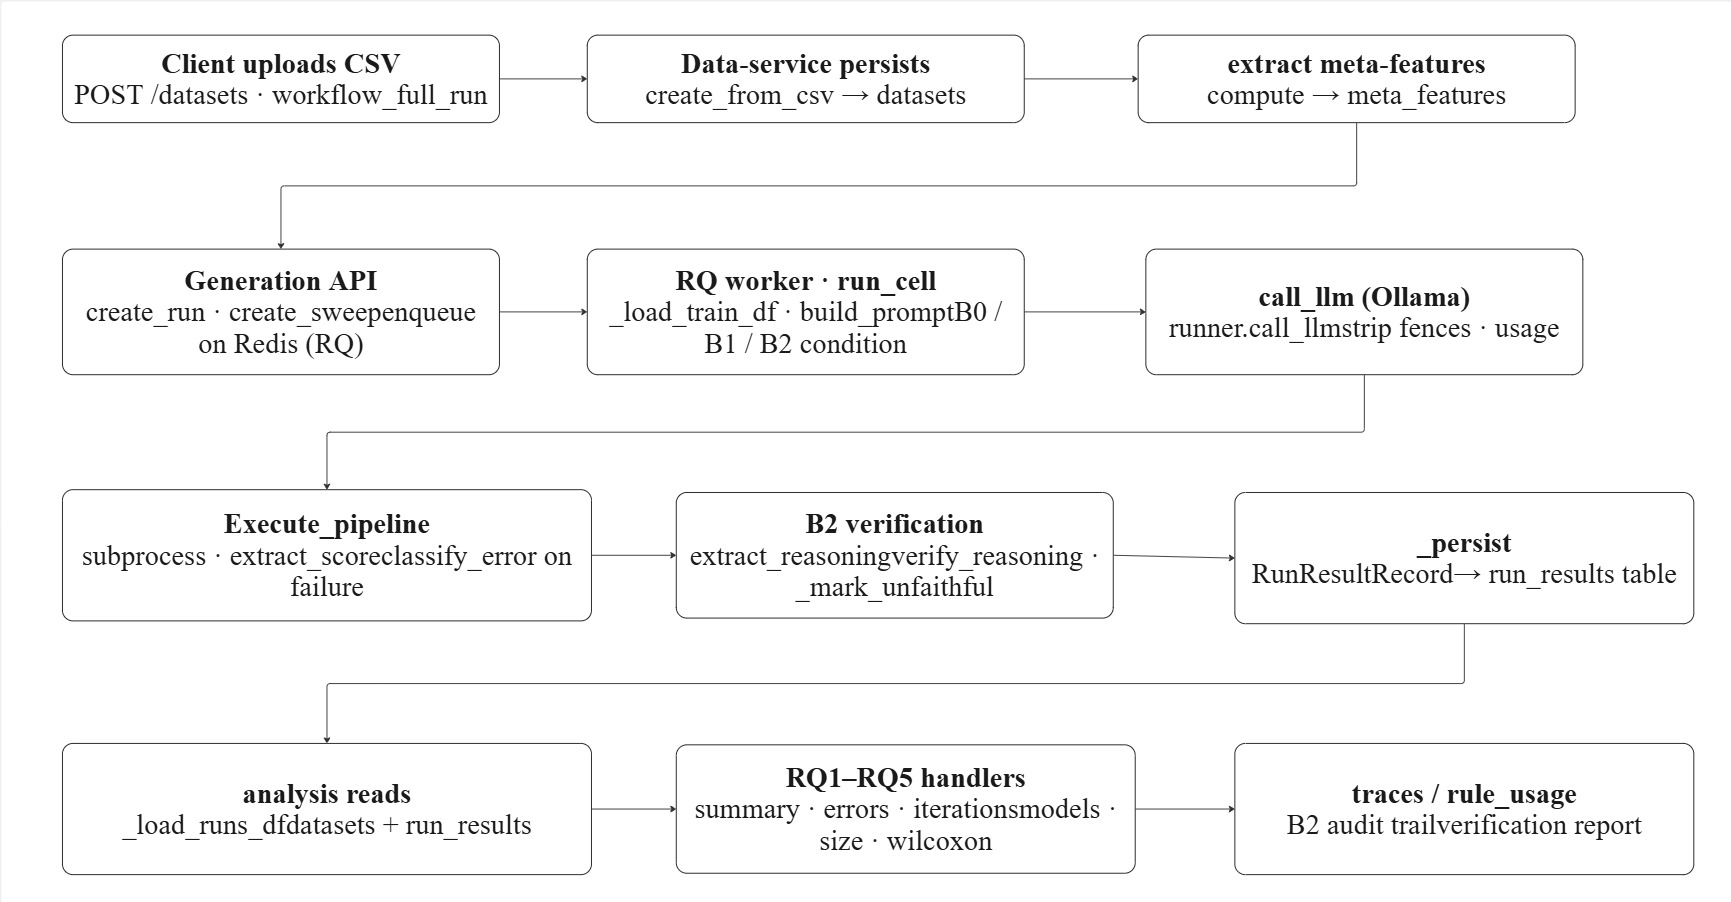
\includegraphics[width=0.84\textwidth]{figures/project_figures/architecture.png}
        \caption{Runtime flow of a single run: upload and meta--feature
        extraction, sweep enqueue, the \texttt{run\_cell} worker (prompt
        build, \texttt{call\_llm}, bounded--subprocess execution, B2
        verification), persistence to \texttt{run\_results}, and the
        read--only RQ1--RQ5 analysis.}
        \label{fig:architecture-flow}
    \end{subfigure}

    \vspace{0.3cm}

    \begin{subfigure}{\textwidth}
        \centering
        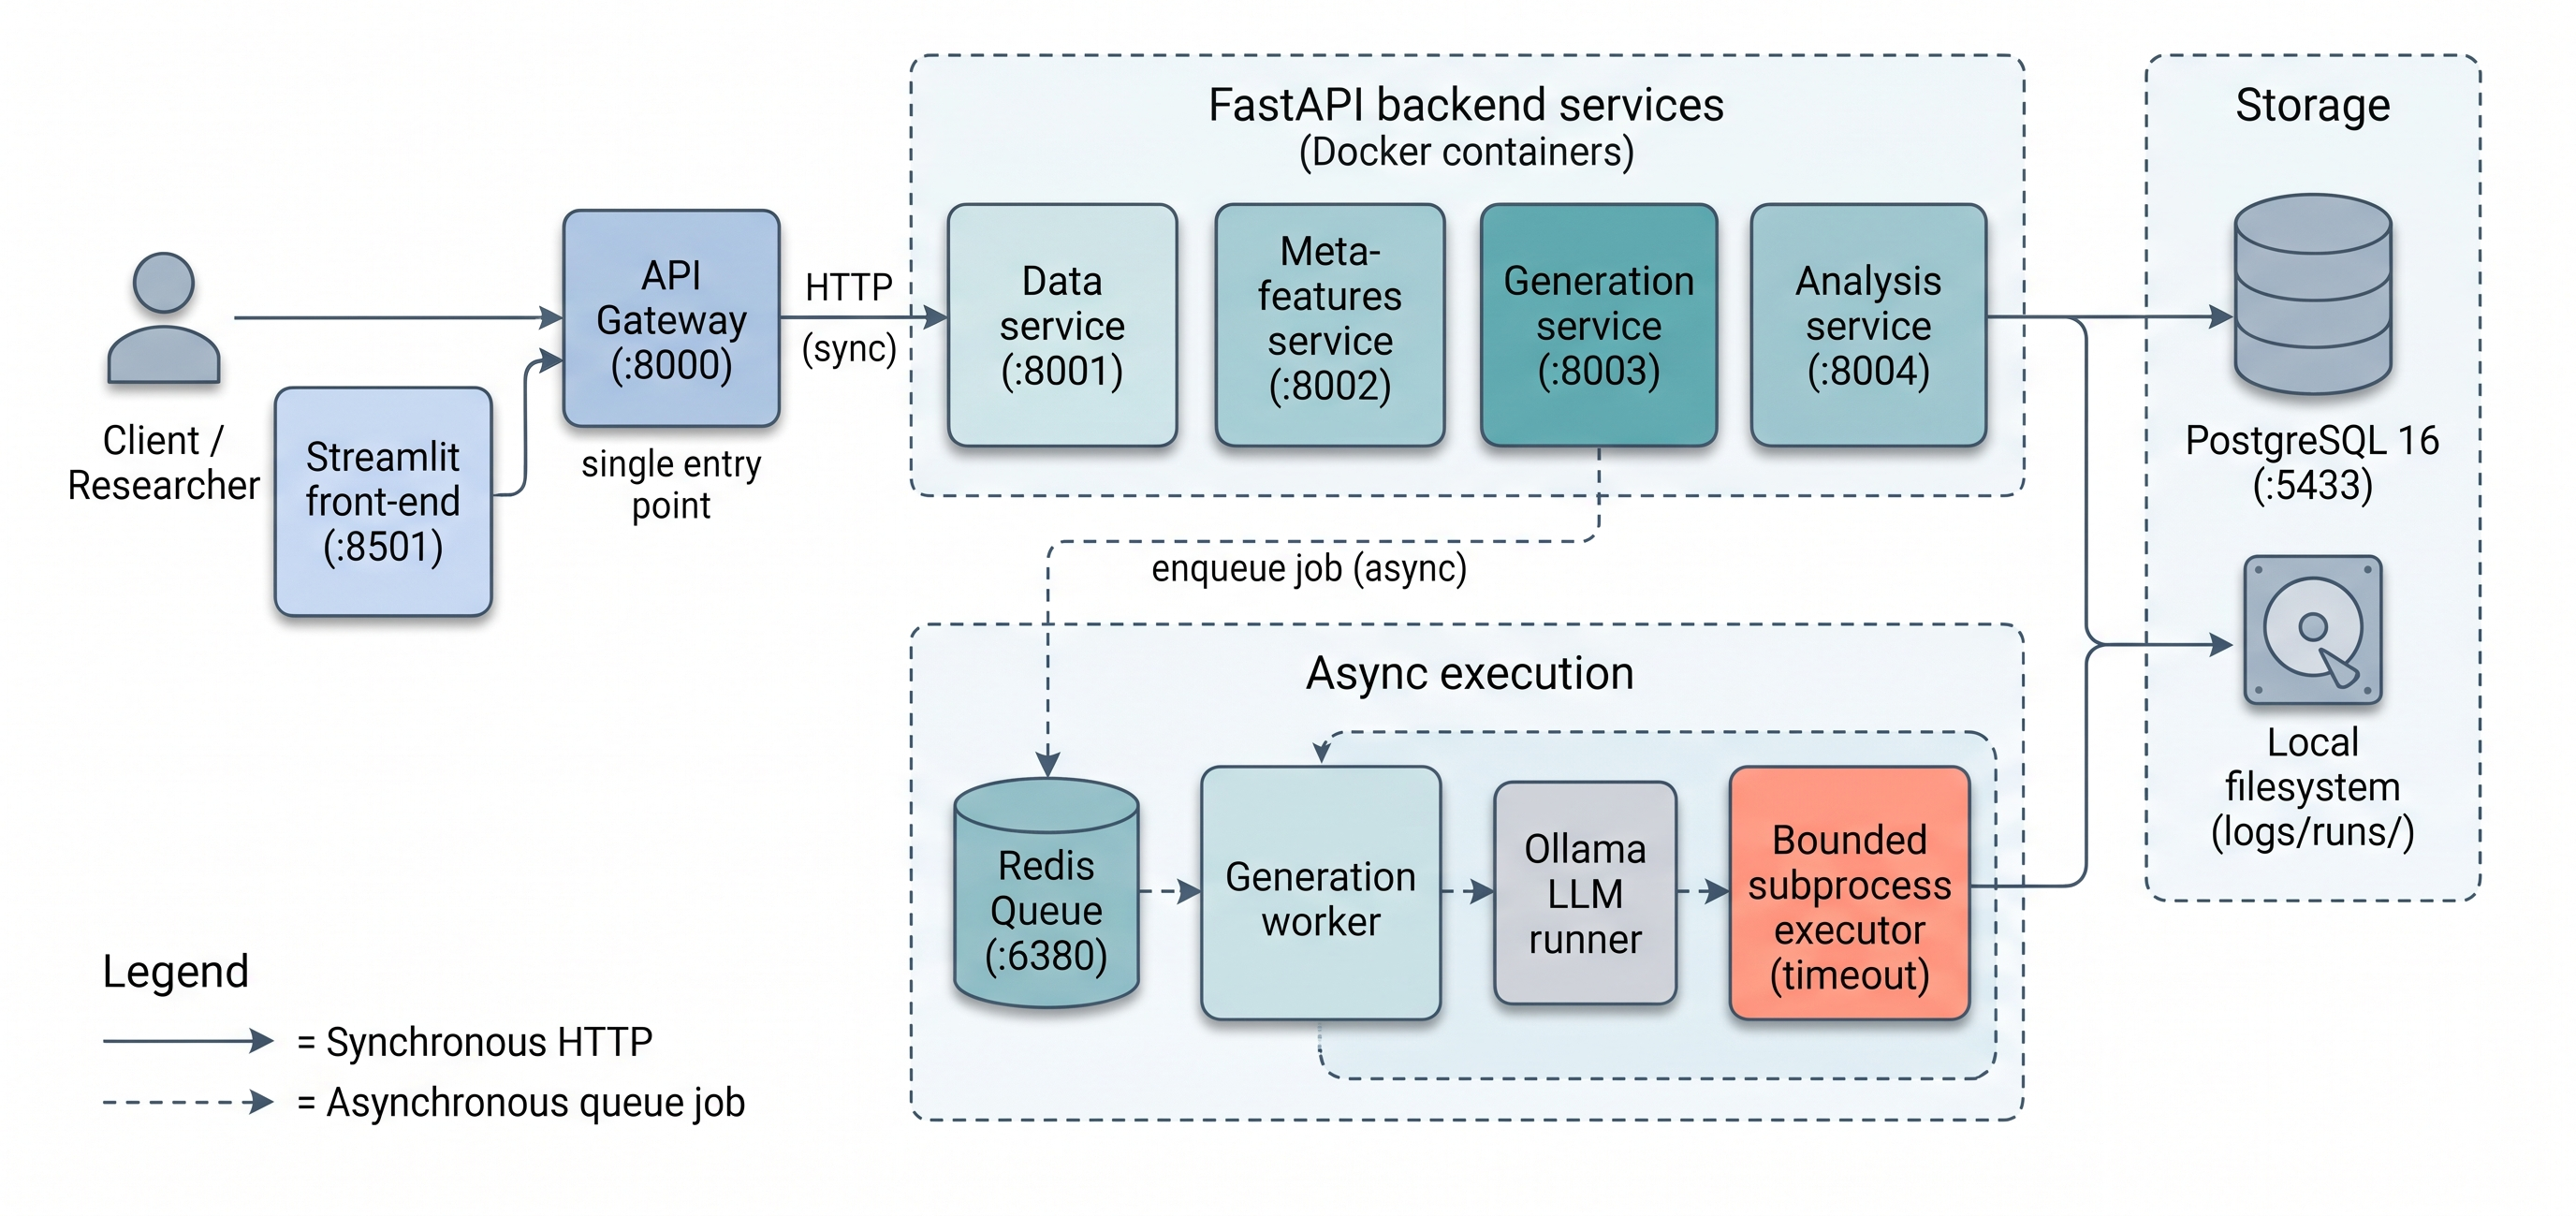
\includegraphics[width=0.84\textwidth]{figures/project_figures/BB_fig_4.1.2.png}
        \caption{Component and deployment view: the Streamlit front--end
        and clients reach the five FastAPI services through the gateway
        (synchronous HTTP); the generation service enqueues jobs on Redis
        for the worker, which drives the Ollama runner and the bounded
        subprocess executor (asynchronous); PostgreSQL and the local
        filesystem hold the results and artefacts. MinIO object storage is
        integrated in the code but was disabled for the reported runs.}
        \label{fig:architecture-components}
    \end{subfigure}
    \caption{System architecture: (a) the runtime flow of one run, and
    (b) the deployed components and their connections.}
    \label{fig:architecture}
\end{figure}

\subsection{Ingestion and Generation Tier}

The ingestion and generation tier exposes HTTP interfaces backed by
\textbf{FastAPI} services (served by \texttt{uvicorn}). A client
uploads a CSV via \texttt{POST /datasets} on the data service and
triggers a full workflow via the gateway. The data service persists
the dataset into the \texttt{datasets} table; the meta--features
service computes and caches the dataset's meta--feature profile into
the \texttt{meta\_features} table, keyed one--to--one by dataset. The
generation service then records a \texttt{sweep\_jobs} row and
enqueues one job per cell on the \textbf{Redis Queue (RQ)}. Note that
``RQ'' here denotes the Redis Queue job runner; the research
questions of this project are written \textbf{RQ1--RQ5} and are a
separate concept.

\subsection{Run and Verification Tier}

The run and verification tier is driven by a \textbf{Redis Queue (RQ)
worker} that executes the \texttt{run\_cell} task. The worker loads
the training dataframe, builds the generation prompt for one of the
three prompt conditions (\texttt{B0}, \texttt{B1}, \texttt{B2}) and
calls the configurable LLM runner (reached through
\texttt{call\_llm\_with\_usage}; the reported runs used hosted Ollama
cloud models), recording token usage.

The emitted pipeline is executed inside a bounded Python subprocess
(a separate process under a wall--clock timeout --- not container-level
isolation) that captures stdout and stderr, extracts the achieved score,
classifies failures into one of thirteen error categories and
preserves failed outcomes. For \texttt{B2} runs a verification stage
follows: the \textbf{implemented verifier} parses the reasoning trace
and, for each cited decision, checks that the named action appears in
the generated code's AST and that the cited statistic matches the
real meta--feature, yielding a boolean \texttt{faithful} verdict that
is persisted. The richer three--valued verdict with mismatch category
and source span specified in Chapter~\ref{ch:method} is the proposed
design; it is not produced by the current tier (see
Chapter~\ref{ch:impl}).

\subsection{Analysis Tier}

The analysis tier persists one \texttt{RunResultRecord} per cell into
the \texttt{run\_results} table. A set of RQ1--RQ5 handlers reads
\texttt{load\_runs}, \texttt{df}\_\texttt{datasets} and \texttt{run\_
results} and produces summaries, error counts, iteration models,
size versus wall--clock curves and the verification report that
answers the research questions. B2 audit trails are retained so that
any aggregate claim can be traced back to the individual verifier
decisions that produced it.

\section{System Workflow}

A single workflow proceeds along the three rows of
Fig.~\ref{fig:architecture-flow} as follows:

\begin{enumerate}
    \item \textbf{Request.} The client calls \texttt{POST
    /datasets} with a CSV and \texttt{POST /workflow\_full\_run}
    with the task specification. The data service persists the file
    and enqueues meta--feature extraction.
    \item \textbf{Sweep creation.} The generation service records a
    \texttt{sweep\_jobs} row and enqueues one job per cell on the
    Redis Queue.
    \item \textbf{Reasoning + code generation.} The RQ (Redis Queue)
    worker loads the training frame, selects the prompt condition
    (B0/B1/B2), calls the LLM runner and receives the generated
    pipeline code (and, under B2, a reasoning trace).
    \item \textbf{Execution.} \texttt{Execute\_pipeline} runs the
    code in a bounded subprocess, times out on hangs, and extracts the
    achieved score.
    \item \textbf{Verification (B2).} The implemented verifier checks
    each decision in the reasoning trace for action presence and
    meta--feature value grounding and records a boolean faithfulness
    verdict; the full RIR/PIR per--claim verdicts of
    Chapter~\ref{ch:method} are the proposed extension.
    \item \textbf{Persistence.} \texttt{\_persist} writes the run
    record (plan, code, trace, score, verdicts) to
    \texttt{run\_results}.
    \item \textbf{Analysis.} The RQ handlers aggregate the stored
    records into the summary, error, iteration, model--class, size
    and wildcard tables, and the trace/rule--usage report.
\end{enumerate}

\section{Use Case Diagram}

The three principal use cases are:

\begin{itemize}
    \item \emph{Submit workflow} --- a researcher uploads a dataset
    and a task specification, selects which research questions to
    exercise, and starts a sweep.
    \item \emph{Audit a run} --- a researcher opens a single run,
    inspects its code, execution trace and (for \texttt{B2}) the
    faithfulness verdict together with the reasons recorded for any
    failed check.
    \item \emph{Reproduce an analysis} --- a researcher regenerates
    the aggregate tables for RQ1--RQ5 from the stored run records,
    without re--running the LLM.
\end{itemize}

\begin{figure}[H]
    \centering
    \miroplaceholder[0.8\textwidth]{figures/project_figures/usecase.png}{%
    Use--case diagram with the actor ``Researcher'' and the three use
    cases: \emph{Submit workflow} (upload dataset + task, start a
    sweep), \emph{Audit a run} (inspect one run's plan, code, trace
    and faithfulness verdict), and \emph{Reproduce an analysis}
    (regenerate RQ1--RQ5 tables from stored rows without re--calling
    the LLM).}
    \caption{Principal use cases of the system.}
    \label{fig:usecase}
\end{figure}

\section{Data Flow}

Data flows through the system as follows:

\begin{itemize}
    \item CSV uploads enter the data service and are indexed by a
    dataset identifier. Meta--features derived from the dataset are
    stored alongside it.
    \item For each cell in a sweep, the RQ worker reads the training
    dataframe and composes a prompt that includes the dataset
    reference, the task type, and the RQ--specific instructions.
    \item The LLM returns a single, self--contained Python script,
    retained verbatim. Under \texttt{B2} the script, when run, also
    prints a structured reasoning trace (a small JSON object of
    decisions) that is captured from its output. The full PIR of
    Chapter~\ref{ch:method} is proposed and is not built here; the
    implemented check parses the code only into the set of names it
    references.
    \item The subprocess run returns a trace object with stdout, stderr,
    the extracted score (or an error classification) and timing
    data.
    \item For \texttt{B2}, the verifier returns a report whose fields
    are the number of decisions, the number found faithful, a single
    boolean \texttt{faithful} flag, and a per--decision list recording
    the step, the cited action, whether that action is present in the
    code, whether the cited value matched, and human--readable reasons
    for any failure. The richer records with mismatch category,
    severity and source span belong to the proposed design. These
    fields join the code, trace and score into a single
    \texttt{RunResultRecord}.
    \item The analysis handlers consume \texttt{RunResultRecord}s
    only; no handler reaches back into the live LLM, so analyses are
    repeatable from storage.
\end{itemize}

\section{Database Design}

The system of record is \textbf{PostgreSQL~16}, accessed through
SQLAlchemy ORM models. The schema has \emph{four} tables, defined so
that every aggregate report can be rebuilt from raw rows --- the
analysis layer only reads, and never writes derived values back.
Figure~\ref{fig:er} gives the entity--relationship overview and
Figures~\ref{fig:schema-dataset}--\ref{fig:schema-sweep} show the
actual ORM definitions.

\begin{itemize}
    \item \textbf{datasets} --- one row per registered dataset:
    \texttt{id}, \texttt{name}, \texttt{source}
    (\texttt{openml}/\texttt{custom}), \texttt{openml\_id},
    \texttt{target\_col}, \texttt{task\_type}, \texttt{train\_path},
    \texttt{test\_path}, \texttt{n\_rows}, \texttt{n\_cols},
    \texttt{created\_at}.
    \item \textbf{meta\_features} --- one row per dataset (enforced by
    a \texttt{UniqueConstraint} on \texttt{dataset\_id}): the full
    meta--feature profile as a \texttt{JSON} \texttt{features} column,
    plus \texttt{computed\_at}. This is the cache that the B2 prompt
    reads.
    \item \textbf{run\_results} --- one row per executed cell:
    \texttt{dataset\_id}, \texttt{condition}
    (\texttt{B0}/\texttt{B1}/\texttt{B2}), \texttt{llm\_backend},
    \texttt{seed}, \texttt{success}, \texttt{test\_score},
    \texttt{error\_category}, \texttt{iterations\_used},
    \texttt{runtime\_seconds}, \texttt{generated\_code\_path},
    \texttt{prompt\_tokens}, \texttt{completion\_tokens}, and ---
    for B2 only --- the \texttt{reasoning\_trace} and
    \texttt{verification\_report} as \texttt{JSON}.
    \item \textbf{sweep\_jobs} --- one row per enqueued sweep:
    \texttt{rq\_job\_id}, \texttt{status}, the cross--product
    \texttt{params} (\texttt{JSON}), and \texttt{total\_cells} /
    \texttt{completed\_cells} / \texttt{failed\_cells} progress
    counters.
\end{itemize}

Large artefacts (generated code, long traces) are written to the local
filesystem under \texttt{logs/runs/}, with a path reference kept in the
row. The stack also integrates \textbf{MinIO} object storage for these
artefacts, but MinIO was disabled in the evaluated deployment (its
images are no longer publicly pullable), so the reported runs used the
filesystem. Writes are idempotent: re--running a cell refreshes its row
rather than creating duplicates.

\begin{figure}[H]
    \centering
    \miroplaceholder{figures/project_figures/er_diagram.png}{%
    Entity--relationship diagram of the four tables ---
    \texttt{datasets} (1)\,$\rightarrow$\,(1) \texttt{meta\_features},
    \texttt{datasets} (1)\,$\rightarrow$\,(many) \texttt{run\_results},
    and the independent \texttt{sweep\_jobs} queue table --- showing
    primary keys, the \texttt{dataset\_id} foreign keys and the JSON
    columns.}
    \caption{Entity--relationship diagram of the PostgreSQL schema.}
    \label{fig:er}
\end{figure}

\begin{figure}[H]
    \centering
    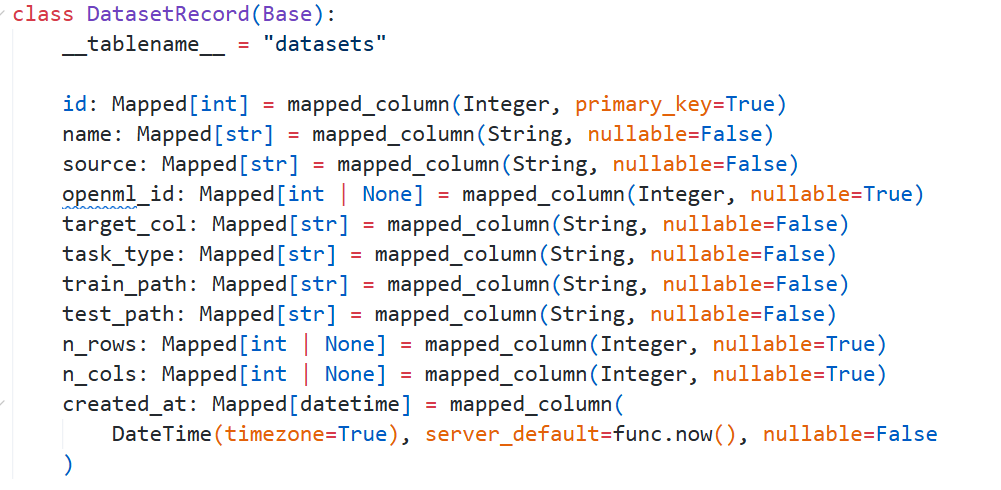
\includegraphics[width=0.92\textwidth]{figures/project_figures/screenshots/DatasetRecord.png}
    \caption{ORM model for the \texttt{datasets} table.}
    \label{fig:schema-dataset}
\end{figure}

\begin{figure}[H]
    \centering
    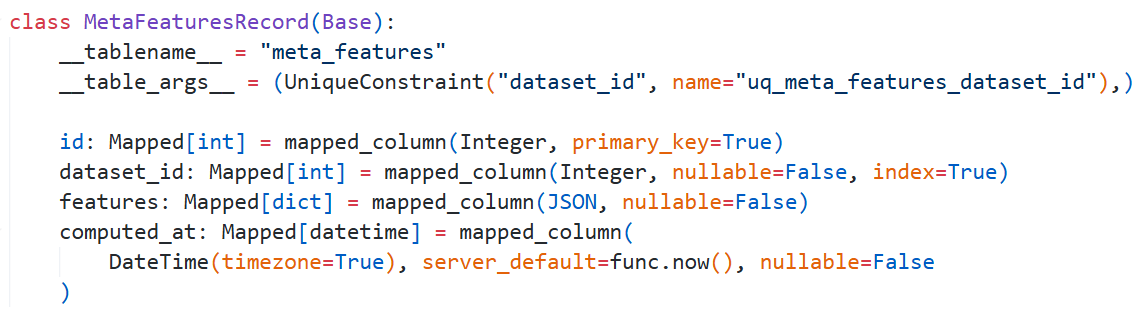
\includegraphics[width=0.92\textwidth]{figures/project_figures/screenshots/MetaFeatures_Schema.png}
    \caption{ORM model for the \texttt{meta\_features} table; the
    \texttt{UniqueConstraint} enforces one profile per dataset.}
    \label{fig:schema-meta}
\end{figure}

\begin{figure}[H]
    \centering
    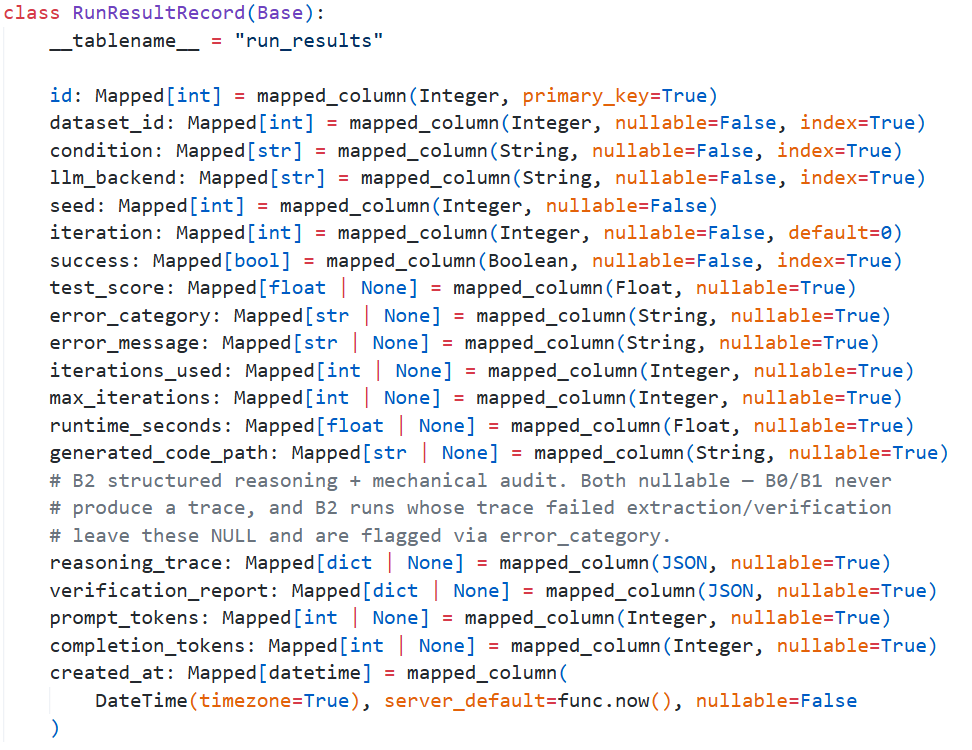
\includegraphics[width=0.92\textwidth]{figures/project_figures/screenshots/RunResultRecord.png}
    \caption{ORM model for the \texttt{run\_results} table; note the
    nullable B2--only \texttt{reasoning\_trace} and
    \texttt{verification\_report} JSON columns and the token counters.}
    \label{fig:schema-run}
\end{figure}

\begin{figure}[H]
    \centering
    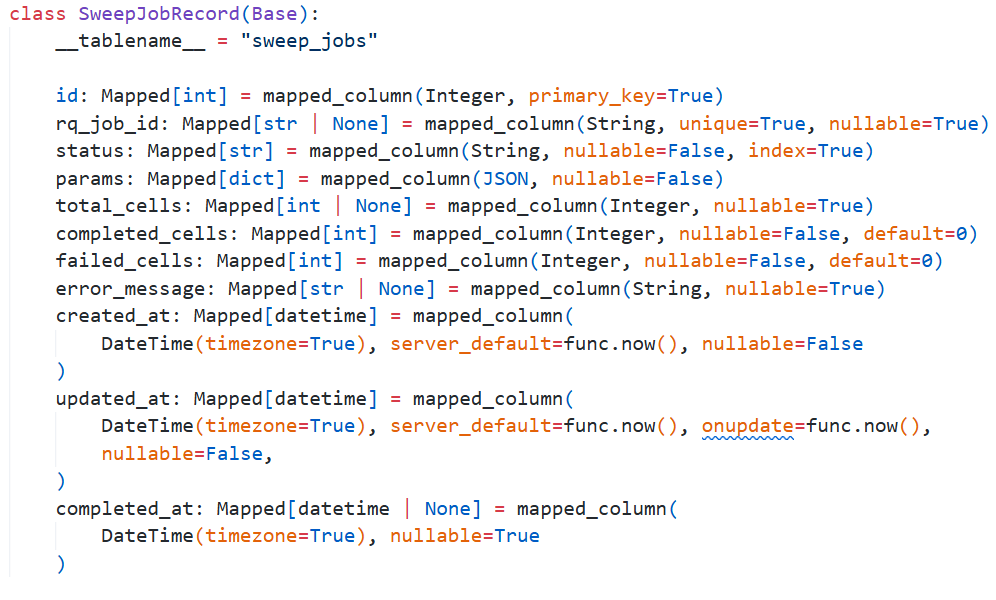
\includegraphics[width=0.92\textwidth]{figures/project_figures/screenshots/SweepJobRecord.png}
    \caption{ORM model for the \texttt{sweep\_jobs} table.}
    \label{fig:schema-sweep}
\end{figure}

\section{Module Description}

The system decomposes into eight modules.

\begin{enumerate}
    \item \textbf{Data Service.} Persists uploaded CSVs, extracts
    and stores meta--features, and exposes \texttt{create\_from\_csv}.
    \item \textbf{Generation API.} Orchestrates \texttt{create\_run}
    and the per--RQ sweep creation on Redis.
    \item \textbf{Prompt Builder.} Constructs the plan--emission and
    code--emission prompts for prompt classes \texttt{B0},
    \texttt{B1}, \texttt{B2} and conditional variants.
    \item \textbf{LLM Runner.} Wraps the configurable LLM backend
    (the reported runs used Ollama) as \texttt{runner.call\_llm} with
    explicit input/output fences and usage accounting.
    \item \textbf{Executor.} The \texttt{Execute\_pipeline} bounded
    subprocess executor that runs the generated code, extracts the
    score, classifies errors on failure and times out hangs.
    \item \textbf{Verifier.} The B2 module that checks, for each cited
    decision, action presence in the code and meta--feature value
    grounding, recording a boolean faithfulness verdict. Lowering the
    plan into the RIR and the code into the PIR to emit the per--claim
    verdicts of Chapter~\ref{ch:method} is the proposed extension and
    is not implemented in this project.
    \item \textbf{Persistence Layer.} \texttt{\_persist} writes the
    \texttt{RunResultRecord} and keeps the audit trail required for
    reproducibility.
    \item \textbf{Analysis Handlers.} RQ1--RQ5 handlers that render
    the summary, error, iteration, model, size and wildcard tables,
    together with the B2 audit/verification report.
\end{enumerate}
